\section{Use-Case 2: Road Warrior} \label{Use-Case 2: Road Warrior}
\subsection{Umsetzung: Kerntätigkeiten}

In AWS und Azure wurden via Terraform die virtuellen Maschinen VyOS aus den jeweiligen Marketplaces installiert.\\
Es wurden für die Cloud-Standorte AWS und Azure analog zu Use-Case 1 Templates erstellt, um den Client-VPN-Konzentrator zu konfigurieren. In der Terraform Resource \textit{azurerm\_linux\_virtual\_machine} wird das richtige VyOS-Image aus dem Cloud-Marketplace referenziert über \textit{source\_image\_reference} und lässt dieses installieren (s. Listing \ref{tf-azure-vyos-machine-image}). Einige dieser Market\-place-Images bieten verschiedene Support- und Lizenz-Verträge an. Über den \textit{plan \{\}}-Kontext wird der passende \textit{Contract} ausgewählt (hier: \glqq Standard support\grqq{}). Ähnlich wurde für die AWS-Instanz vorgegangen. 
%TC:ignore
\begin{listing}[h]
\begin{minted}[breaklines,frame=single]{tf}
resource "azurerm_linux_virtual_machine"  "azurerm_linux_virtual_machine" {
  name = "vyos-test"
  location = var.rg_location
  resource_group_name = var.rg_name
  admin_username = "vyos"
  size = "Standard_B1s"
  network_interface_ids = [ azurerm_network_interface.azurerm_network_interface.id ]
  os_disk {
    caching = "ReadWrite"
    storage_account_type = "Premium_LRS"
  }
  admin_ssh_key {
    username   = "vyos"
    public_key = file("~/.cred_mgmt/_push/authorized_keys/id_rsa_automation.pub")
  }
  source_image_reference {
    publisher = "sentriumsl"
    offer = "vyos-1-2-lts-on-azure"
    version = "latest"
    sku = "vyos-1-2-crux"
  }
  plan {
    name = "vyos-1-2-crux"
    product = "vyos-1-2-lts-on-azure"
    publisher = "sentriumsl"
  }
}
\end{minted}
\caption{Suche und Installation des VyOS-Images in Azure}
\label{tf-azure-vyos-machine-image}
\end{listing}\FloatBarrier
%TC:endignore
Public/Private-Schlüsselpaar wurde vorab erstellt, von der pfSense-PKI signiert und mit dem Zertifikat auf dem Terraform-Server gespeichert. Während des Terraform-\gls{Deployment}s wird Private Key und Zertifikat per Terraform Provisioner auf das Zielsystem kopiert. Sie werden in der Config dann via \textit{set interfaces openvpn vtun0 tls cert-file / key-file} referenziert.\\
In der Praxis sollte darauf verzichtet werden, das Schlüsselmaterial \glqq auf einem anderen System vorzulagern\grqq{}: Ein privater Schlüssel sollte nur auf dem Server erzeugt und gespeichert werden, auf dem dieser final genutzt wird. Optimalerweise wäre dies zur Laufzeit der Terraform-\gls{Deployment}s. Zur Vereinfachung des Use-Cases wurde auf diesen Schritt verzichtet. Eine Möglichkeit zur automatisierten Signatur von vertrauenswürdigen Zertifikaten ist das Simple Certificate Enrollment Protocol (SCEP)\cite[S.554]{Schmeh2013}.\\
Für den sich verbindenden Roadwarrior-Client sind diverse Konfigurationen hinterlegt: Suchdomäne, (interner) Name-Server und Routen, die über den VPN-Konzentrator erreicht werden können (s. Listing \ref{vpn-c2s-server-config}).
Weiterhin wird ein MSS-Clamping (s. Kapitel \ref{mtumss}) vorgenommen, um IP-Fragmen\-tierung von TCP-Applikationen möglichst zu verhindern.\\
Das Subnetz, in dem die OpenVPN-Clients terminiert werden, wird wieder dynamisch aus dem IPAM alloziert.
%TC:ignore
\begin{listing}[h]
\begin{minted}[breaklines,frame=single]{text}
set interfaces openvpn vtun0 openvpn-option "--mssfix 1350"
set interfaces openvpn vtun0 server domain-name 'intern.ba.mungard.de'
set interfaces openvpn vtun0 server name-server '192.168.201.1'
set interfaces openvpn vtun0 server push-route '10.32.0.0/16'
set interfaces openvpn vtun0 server push-route '10.33.0.0/16'
set interfaces openvpn vtun0 server push-route '192.168.201.0/24'
set interfaces openvpn vtun0 server subnet ${aws_vpn_clients_subnet}/${aws_vpn_clients_subnet_mask}
set interfaces openvpn vtun0 tls ca-cert-file '/config/auth/BA_CA_2021.crt'
set interfaces openvpn vtun0 tls cert-file '/config/auth/vpn-server-aws.ba.mungard.de.crt'
set interfaces openvpn vtun0 tls dh-file '/config/auth/dh2048.pem'
set interfaces openvpn vtun0 tls key-file '/config/auth/vpn-server-aws.ba.mungard.de.key'
\end{minted}
\caption{Terraform Template für VyOS OpenVPN-Server in AWS}
\label{vpn-c2s-server-config}
\end{listing}
%TC:endignore

Die drei Cloud-Standorte wurden in diesem Proof-of-Concept verteilt über verschiedenen Regionen: Dublin (Azure), Frankfurt (AWS), Kiel (Private Cloud). Es werden drei Roadwarrior-Clients simuliert, die ebenso am jeweiligen Standort stehen. Dazu wurden weitere VMs an den Cloud-Standorten hochgefahren: Sie wurden völlig isoliert von dem restlichen \gls{Deployment} installiert und sind nicht Teil der internen Netzwerke 10.32.0.0/16 bzw. 10.33.0.0/16 (s. Listing \ref{ext-ip-addr-roadwarrior}). Zugang zu internen Ressourcen wird nur über eine erfolgreiche Authentifizierung am VPN-Konzentrator gewährleistet.
%TC:ignore
\begin{listing}[h]
\begin{minted}[breaklines,frame=single]{bash}
ubuntu@vpn-client-azure:~$ ip -brief -4 address show | grep -v lo
eth0             UP             10.42.0.4/24

\end{minted}
\caption{IP-Adresse in CIDR-Notation des Roadwarrior-Clients}
\label{ext-ip-addr-roadwarrior}
\end{listing}\FloatBarrier
%TC:endignore
Internet-Traffic ist möglich, Zugriff auf interne Ressourcen ist nicht möglich (s. Listing \ref{internet-access-roadwarrior}). 192.168.201.1 ist eine IP-Adresse der Private Cloud.
%TC:ignore
\begin{listing}[h]
\begin{minted}[breaklines,frame=single]{text}
#Internet-Traffic
ubuntu@vpn-client-azure:~$ ping -c 1 8.8.8.8
PING 8.8.8.8 (8.8.8.8) 56(84) bytes of data.
64 bytes from 8.8.8.8: icmp_seq=1 ttl=112 time=0.987 ms

--- 8.8.8.8 ping statistics ---
1 packets transmitted, 1 received, 0% packet loss, time 0ms
rtt min/avg/max/mdev = 0.987/0.987/0.987/0.000 ms

#Interne Adresse ist nicht erreichbar 
ubuntu@vpn-client-azure:~$ ping -c 1 192.168.201.1
PING 192.168.201.1 (192.168.201.1) 56(84) bytes of data.

--- 192.168.201.1 ping statistics ---
1 packets transmitted, 0 received, 100% packet loss, time 0ms

\end{minted}
\caption{Kein Zugriff des Roadwarrior-Clients auf interne Ressourcen ohne VPN-Verbindung}
\label{internet-access-roadwarrior}
\end{listing}\FloatBarrier
%TC:endignore
Die MaxMind GeoIP-Datenbank wurde auf dem DNS-Server installiert und in der Bind-Konfiguration referenziert (s. Listing \ref{bind-geoip-directory}).
%TC:ignore
\begin{listing}[h]
\begin{minted}[breaklines,frame=single]{bash}

$ grep -E 'options|geoip-directory|^};' < named.conf.options
options {
        geoip-directory "/usr/share/GeoIP";
};

\end{minted}
\caption{Konfiguration GeoIP für Bind-Nameserver}
\label{bind-geoip-directory}
\end{listing}\FloatBarrier
%TC:endignore
Dadurch wurde ermöglicht, GeoIP-Daten in einer Access Control List (ACL) zu nutzen und verschiedene Fälle zu definieren. Die ACL heißt in diesem Falle \glqq dublin\grqq{} und erlaubt Zugriffe aus der Stadt Dublin bzw. Zugriff für den TSIG-Key \glqq db-vpn.ba.mungard.de\grqq{} (s. Listing \ref{tsig-key-acl}). Dieser Key wird benötigt, um Zonen-Updates machen zu können und ist im entsprechenden Terraform-Modul hinterlegt.
%TC:ignore
\begin{listing}[h]
\begin{minted}[breaklines,frame=single]{text}
acl "dublin" {
        geoip city Dublin;
        key "db-vpn.ba.mungard.de.";
};
\end{minted}
\caption{ACL \glqq dublin\grqq{} für GeoIP und TSIG-Key}
\label{tsig-key-acl}
\end{listing}\FloatBarrier
%TC:endignore
Weiterhin existiert ein \textit{View} \glqq Dublin\grqq{}, in dem die ACL und Zonen-Daten zusammengeführt werden (s. Listing \ref{view-dublin-bind}). Mit \textit{allow-update} werden Zonen-Updates explizit und ausschließlich für genannten TSIG-Key erlaubt.
%TC:ignore
\begin{listing}[h]
\begin{minted}[breaklines,frame=single]{text}
view "dublin" {
        match-clients { dublin; };
        zone "ba.mungard.de" {
                type master;
                file "/etc/bind/ba_zones/db.geo.ba.mungard.de-dublin";
                allow-update { key "db-vpn.ba.mungard.de."; };
        };
};
\end{minted}
\caption{View \glqq dublin\grqq{} für Zusammenführung von ACL und Zonendatei}
\label{view-dublin-bind}
\end{listing}\FloatBarrier
%TC:endignore
In der Zonen-Datei für Dublin befindet sich vor dem Terraform-\gls{Deployment} nur ein A-Record \textit{default-vpn}. Dies ist der A-Record, der als Fallback dient (s. Listing \ref{zone-dublin-before-deployment}). Gemäß Evaluationskriterien muss ein Roadwarrior-Client auf die Private Cloud zurückfallen, wenn bisher kein \gls{Deployment} stattgefunden hat. Die öffentlich auflösbare Zone lautet \textit{ba.mungard.de}.
%TC:ignore
\begin{listing}[h]
\begin{minted}[breaklines,frame=single]{bash}
$ grep -A1 "ORIGIN ba.mungard.de" < /etc/bind/ba_zones/db.geo.ba.mungard.de-dublin
$ORIGIN ba.mungard.de.
default-vpn             A       195.244.254.197
\end{minted}
\caption{Die Zone ba.mungard.de vor dem Terraform-\gls{Deployment}}
\label{zone-dublin-before-deployment}
\end{listing}\FloatBarrier
%TC:endignore
Die Konfigurationen für Frankfurter und Kieler Clients wurden analog vollzogen. Dies gilt ebenso für das interne DNS. Allerdings wird hier kein GeoIP genutzt, sondern anhand der Absender-IP-Adresse wird eine ACL (hier \glqq dublin-internal\grqq{}) \textit{getroffen} (s. Listing \ref{view-internal-bind}). Auch die internen Zonen sind durch Terraform via DNS UPDATE editierbar (key \glqq db-vpn-internal.ba.mungard.de.\grqq{}).
%TC:ignore
\begin{listing}[h]
\begin{minted}[breaklines,frame=single]{text}
acl "dublin-internal" {
        10.32.0.0/16;
        key "db-vpn-internal.ba.mungard.de.";
};
\end{minted}
\caption{ACL \glqq dublin-internal\grqq{} für internes DNS}
\label{view-internal-bind}
\end{listing}\FloatBarrier
%TC:endignore
Weiterhin gibt es eine ACL \glqq match-all\grqq{}, welche für anfragende Clients vorgesehen ist, die nicht per GeoIP identifiziert werden. Durch das Netzwerk 0.0.0.0/0 treffen die ACL alle restlichen Teilnehmer des Internets (s. Listing \ref{view-matchall-bin}).
%TC:ignore
\begin{listing}[h]
\begin{minted}[breaklines,frame=single]{text}
acl "match-all" {
        0.0.0.0/0;
        key "all-vpn.ba.mungard.de.";
};
\end{minted}
\caption{ACL \glqq match-all\grqq{} für alle übrigen Anfragen}
\label{view-matchall-bin}
\end{listing}\FloatBarrier
%TC:endignore

Im Terraform-Modul muss ein Provider \textit{pro} TSIG-Key konfiguriert werden. Der server-Parameter konfiguriert den Nameserver, der per DNS UPDATE editiert werden soll. Außerdem ist das Pre-Shared-Secret (TSIG-Key) hinterlegt. Es wird für die Domain vpn.ba.mungard.de die IP-Adresse (\textit{var.dublin\_ip}) des VPN-Konzentrators in Dublin (Azure) eingetragen, welche dynamisch zur Laufzeit entsteht (s. Listing \ref{tf-provider-dns}).
%TC:ignore
\begin{listing}[h]
\begin{minted}[breaklines,frame=single]{tf}
provider "dns" {
  alias = "dns-dublin"
  update {
    server        = "192.168.200.29"
    key_name      = "db-vpn.ba.mungard.de."
    key_algorithm = "hmac-sha256"
    key_secret    = "9jzMaHwILwTzx9b/Ws8RAfBwC+eJpjOI2hEmAgCjV/4="
  }
}
resource "dns_a_record_set" "vpn-dublin" {
  provider = dns.dns-dublin
  zone = "ba.mungard.de."
  name = "vpn"
  addresses = [ var.dublin_ip ]
  ttl = 15
}
\end{minted}
\caption{Terraform Modul zur Veränderung von DNS-Zonen}
\label{tf-provider-dns}
\end{listing}\FloatBarrier
%TC:endignore
Nach dem Terraform-\gls{Deployment} kann man sich per \texttt{rndc dumpdb -zones} alle Views ausgeben lassen (hier gefiltert auf die relevantesten Einträge der Views \glqq dublin\grqq{} und \glqq match-all\grqq{}). Man erkennt in Listing \ref{bind-entries-after-tf}, dass in beiden Views für die Domain default-vpn.ba.mungard.de die gleiche IP (\glqq Fallback\grqq{}) zurückgegegeben.\\
Für Domain vpn.ba.mungard.de ist im View \glqq dublin\grqq{} nur eine Azure-IP sichtbar, während im View \glqq match-all\grqq{} IPs aller VPN-Konzentratoren des \gls{Deployment}s vorkommen.
%TC:ignore
\begin{listing}[h]
\begin{minted}[breaklines,frame=single]{bash}
$ grep -E -A12 'Start view (dublin|match-all)$' < /var/cache/bind/named_dump.db | grep -Ev '(client|SOA|NS|nu|^;$)'
; Start view dublin
; Zone dump of 'ba.mungard.de/IN/dublin'
default-vpn.ba.mungard.de.          15 IN A           195.244.254.197
vpn.ba.mungard.de.                  15 IN A           137.116.237.246
; Start view nu
--
; Start view match-all
; Zone dump of 'ba.mungard.de/IN/match-all'
default-vpn.ba.mungard.de.          15 IN A           195.244.254.197
vpn.ba.mungard.de.                  15 IN A           18.197.9.208
vpn.ba.mungard.de.                  15 IN A           137.116.237.246
vpn.ba.mungard.de.                  15 IN A           195.244.254.197

\end{minted}
\caption{View \glqq dublin\grqq{} und View \glqq match-all\grqq{}}
\label{bind-entries-after-tf}
\end{listing}\FloatBarrier
%TC:endignore

Listing \ref{zone-dump-dublin-internal} zeigt einen exemplarischen Zone-Dump für einen internen Client, welcher über Dublin verbunden ist. Die interne Zone ist intern.ba.mungard.de. Alle Cloud-Standorte nutzen den gleichen Name-Server (ns1.intern.ba.mungard.de), welcher in der Private Cloud vorhanden ist.\\
%TC:ignore
\begin{listing}[h]
\begin{minted}[breaklines,frame=single]{bash}
$ grep -E -A10 'Start view dublin-internal' < /var/cache/bind/named_dump.db | grep -Ev '(client|SOA|NS|^;$)'
; Start view dublin-internal
; Zone dump of 'intern.ba.mungard.de/IN/dublin-internal'
ns1.intern.ba.mungard.de.             15 IN A           192.168.201.1
www.intern.ba.mungard.de.             15 IN A           10.32.0.4
\end{minted}
\caption{Zone-Dump der internen Zone intern.ba.mungard.de (Standort: Dublin)}
\label{zone-dump-dublin-internal}
\end{listing}\FloatBarrier
%TC:endignore
Es wurde eine Ubuntu-VM pro Standort (hier Azure in Dublin) via Terraform bereitgestellt. Per remote-exec provisioner wird das Apache2-Paket installiert und die Default-HTML-Seite (\glqq It works!\grqq{}) per \texttt{sed} manipuliert. Damit im Web-Browser der Standort sofort ersichtlich sein, von dem die HTML-Seite ausgeliefert wurde. Analoge Konfiguration hat für den Standort AWS in Frankfurt stattgefunden.
%TC:ignore
\begin{listing}[h]
\begin{minted}[breaklines,frame=single]{tf}
resource "null_resource" "www_config" {
  depends_on = [ azurerm_virtual_machine.azurerm_virtual_machine ]
  connection {
    type = "ssh"
    host = azurerm_network_interface.azurerm_network_interface.private_ip
    user = "ubuntu"
    private_key = file(var.private_key_file)
  }

  provisioner "remote-exec" {
    inline = [
      "sudo apt update",
      "sudo apt install -y apache2",
      "sudo sed -i 's/It works!/It works! @Azure Cloud (Location: \"North Europe - Dublin\")/' /var/www/html/index.html" ]
  }
}
\end{minted}
\caption{Configuration Management nach \gls{Deployment} der virtuellen Maschine per remote-exec Provisioner}
\label{sed-replace-apache-location}
\end{listing}\FloatBarrier
%TC:endignore

Die OpenVPN Client-Konfigurationen wurden vor Terraform-\gls{Deployment} bereits \textit{inline} in einer Textdatei vorbereitet (s. Listing \ref{vpn-c2s-server-config}). Auch hier gilt analog zur Server-Konfiguration, dass Schlüsselmaterial optimalerweise erst zur Laufzeit erstellt wird. Zertifikate und privater Schlüssel wurden im folgenden Beispiel gefiltert. Von zentraler Bedeutung sind Zeilen 1 und 2: Durch mehrfache Angabe einer remote-Direktive kann ein Fallback auf \textit{default-vpn.ba.mungard.de} stattfinden, sollte \textit{vpn.ba.mungard.de} nicht auflösbar sein. Die erste remote-Direktive wird dabei \textbf{immer} zuerst kontaktiert, dann folgt der Fallback auf die zweite.\\
Dies gilt für den Fall, falls das \gls{Deployment} noch nicht stattgefunden hat und der Client nicht in der Nähe von Kiel ist, um per GeoIP-ACL Zugriff auf die Auflösung von \textit{vpn.ba.mungard.de} erhält. Per \textit{pullfilter ignore redirect-gateway} wird verhindert, dass ein Default Gateway über den Tunnel signalisiert wird: Nur alle \textbf{bekannten} Routen kommen über die OpenVPN-Server-Konfiguration. Es findet kein \textit{full tunneling} statt.
%TC:ignore
\begin{listing}[h]
\begin{minted}[linenos,breaklines,frame=single]{text}
remote vpn.ba.mungard.de 61231
remote default-vpn.ba.mungard.de 61231
port 0
pull-filter ignore redirect-gateway
cipher aes-256-cbc
client
dev tun
resolv-retry infinite
remote-cert-tls server
verb 3
persist-tun

\end{minted}
\caption{Die OpenVPN-Client Konfigurationsdatei (gekürzt)}
\label{ovpn-client-conf}
\end{listing}\FloatBarrier
%TC:endignore



\newpage
Analog zu den Kapiteln \ref{xml-tunnel-parameters} bis \ref{azure-deployment-time} werden im Folgenden Probleme und Lösungsfindung erläutert.
\subsection{Beschleunigung des \gls{Deployment}s}\label{accelerate-deployment-use-case-2}
Das Azure VPN Gateway benötigt viel Zeit für die Erstellung (s. Kapitel \ref{azure-deployment-time}). Da Use-Case 2 direkt auf diesem Use-Case aufsetzt, hätte das ebenso eine lange \gls{Deployment}-Zeit nach sich gezogen. So war ursprünglich die Idee, den Programmcode aus Use-Case 1 zu kopieren und um die Infrastruktur-Komponenten aus Use-Case 2 zu ergänzen. Somit hätte sich die \gls{Deployment} Zeit $t_{gesamt}$ aus den jeweiligen \gls{Deployment}-Zeiten der Infrastrukturen aus Use-Case 1 und Use-Case 2 zusammengesetzt:\\
$t_{gesamt} = t_{Infrastruktur_{U1}} + t_{Infrastruktur_{U2}}$

Somit kam die Frage auf, ob man das \gls{Deployment} für Use-Case 2 beschleunigen könnte. Da in Use-Case 2 viele Tests und Änderungen gemacht wurden, musste das \gls{Deployment} oftmals komplett neu erfolgen, was \gls{Deployment}-Zeiten von bis zu anderthalb Stunden (siehe \ref{xml-tunnel-parameters}) nach sich ziehen kann.\\
Dieses Problem konnte mit der Data Source \textit{terraform\_remote\_state} zumindest abgemildert werden\cite{remotestateimport2021}. So wurde die Infrastruktur aus Use-Case 1 als \textbf{vorhanden} angenommen und die Infrastruktur aus Use-Case 2 lediglich hinzugefügt.\\
Der \textit{state import} findet in der Datei \underline{main.tf} von Use-Case 2 statt und referenziert die Datei \underline{terraform.tfstate} aus Use-Case 1.
%TC:ignore
\begin{listing}[h]
\begin{minted}[breaklines,frame=single]{tf}
data "terraform_remote_state" "base_deployment" {
  backend = "local"
  config = {
    path = "../use_case_1/terraform.tfstate"
  }
}

\end{minted}
\caption{Import des Remote States aus Use-Case 1 in Use-Case 2}
\label{tf-remote-state-import}
\end{listing}\FloatBarrier
%TC:endignore
Der Remote-State-Import dauert einen kurzen Moment, wird aber in der folgenden Betrachtung vernachlässigt.
Unter der Annahme, dass Use-Case 1 bereits bereitgestellt wurde, ist die Laufzeit des \gls{Deployment}s effektiv:\\
$t_{gesamt} = t_{Infrastruktur_{U2}}$

Im Allgemeinen hat sich dieser \glqq Teile-und-herrsche\grqq{}-Ansatz im Zusammenspiel mit Terraform als sehr hilfreich erwiesen, um Konsistenz-Probleme der asynchronen Cloud-APIs während der \gls{Deployment}-Phase zu verringern\cite[S.183-184]{Brikman2019}. Probleme während des \gls{Deployment}s entstanden v.a. dann, wenn \glqq zu viele\grqq{} Abhängigkeiten in der Infrastruktur vorhanden waren. Für die Verschaltung von aufgeteilten Terraform-\gls{Deployment}s eignet sich das Werkzeug Terragrunt\cite[S.98]{Brikman2019}.
\newpage
\subsection{More-specific Routing in AWS Route Tables}
Die Roadwarrior Clients müssen in einem eigenen Subnetz \glqq hinter\grqq{} dem VPN-Konzentrator terminiert werden. Dafür werden Routing-Einträge notwendig, damit AWS VPC bzw. Azure VNET die Information besitzen, über welchen \textit{Next-Hop} das Roadwarrior-VPN-Subnetz erreicht werden kann. Durch \textit{Route Tables} stellt dies auch keine Hürde dar in Azure. AWS hingegen bietet keine Möglichkeit, Subnetze mit einer längeren Netzmaske in der Route Table zu hinterlegen, falls sie ein Subnetz des VPC CIDR darstellen würden. Man spricht auch von \glqq more specifics\grqq{}.\\
Im Beispiel von Abb. \ref{grafik:more_specific_not_allowed_aws} sei das VPC CIDR 192.168.0.0/16 (Target: local). Es soll eine Route auf ein Netzwerk 192.168.100.0/24 über die AWS Instance \glqq i-06230ccaa[...]\grqq{} (Next-Hop) gesetzt werden, was eine more specific Route zum VPC CIDR darstellt.
Es wird im AWS Dashboard beim Versuch, eine more-specific Route anzulegen, eine Fehlermeldung ausgegeben.

\begin{figure}[h]
  \centering
  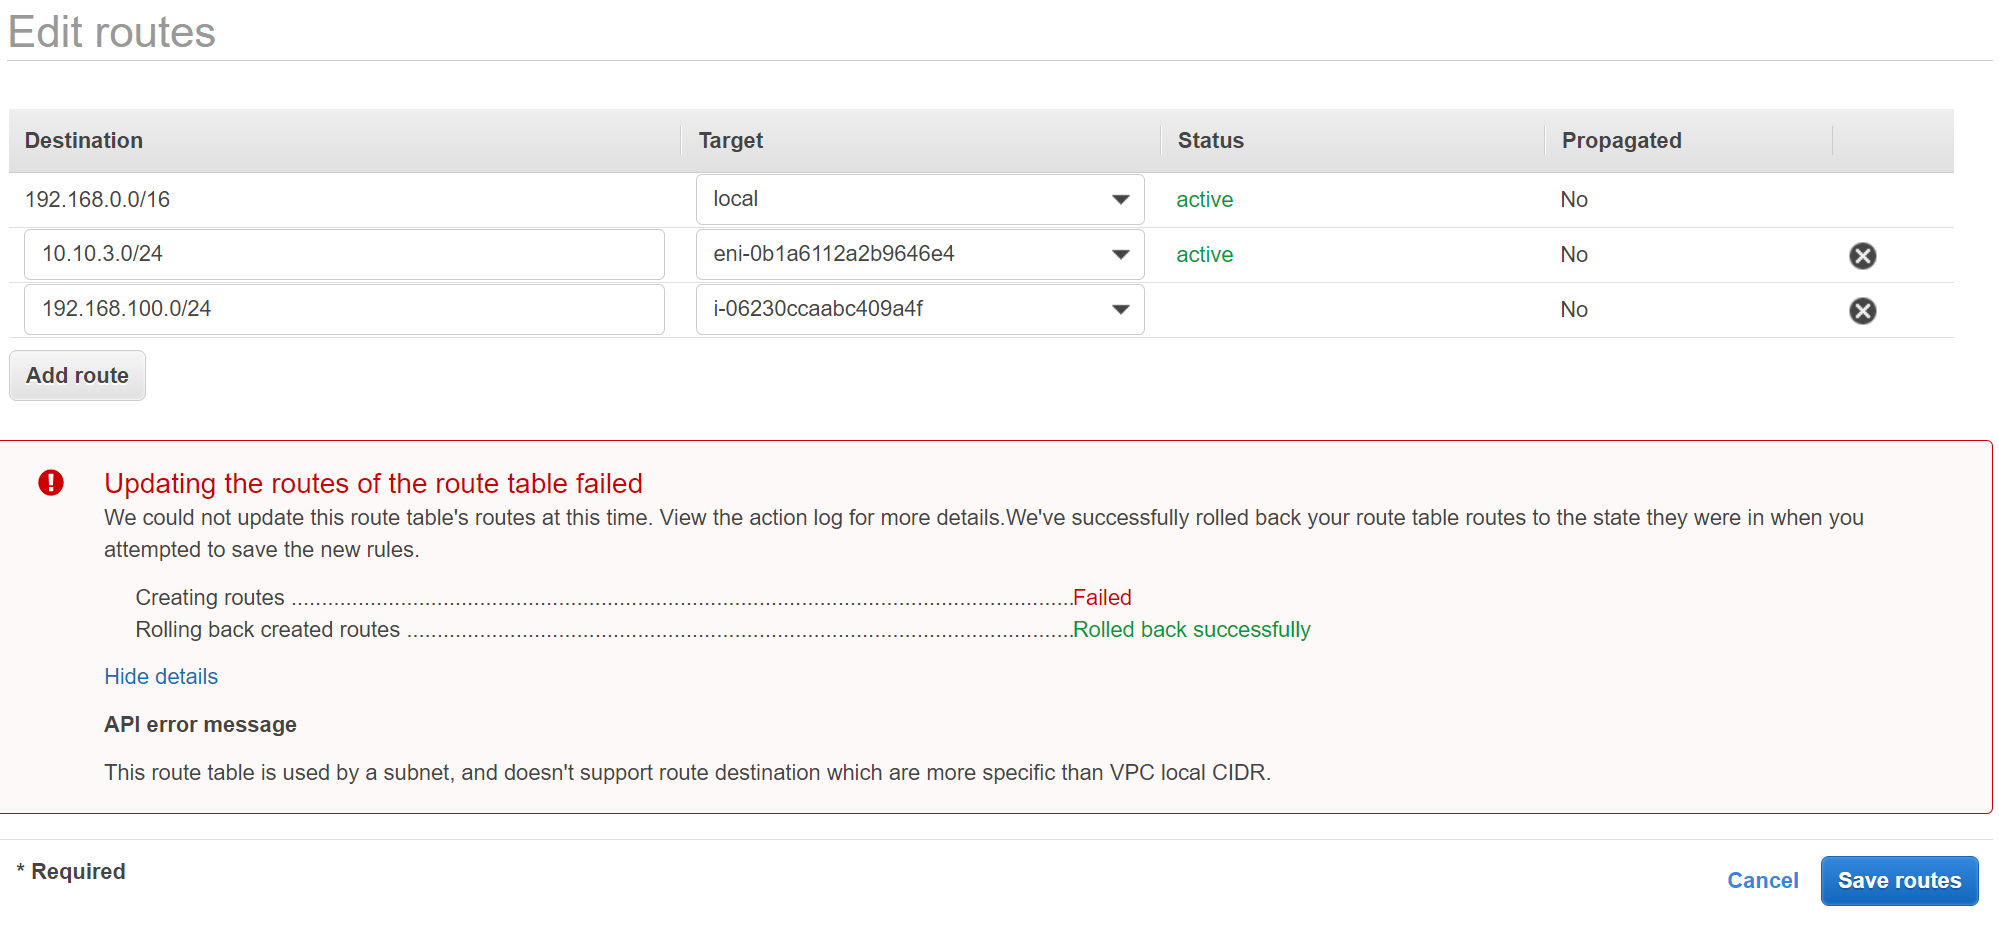
\includegraphics[scale=0.35]{Figures/more_specific_not_allowed_aws.PNG}
  \caption{More-specific Routing ist in AWS Route Tables nicht möglich.}
  \label{grafik:more_specific_not_allowed_aws}
\end{figure}\FloatBarrier
More specific Routing wird laut Amazon User Guide für das \textbf{Main Route Table} nicht unterstützt\cite[S.230]{awsug2020}. Dieser Constraint bezieht sich allerdings auf \textbf{alle} Route Tables, wie weitere Tests zeigten.\\
Präfixe zu nutzen, welche nicht more specific sind, ginge insofern als das Routing \textit{innerhalb} des VPCs möglich wird, allerdings werden diese Präfixe nicht durch BGP den anderen Stellen bekannt gemacht. Somit erreichen Pakete aus Netzwerken, welche nicht im AWS VPC \glqq leben\grqq{}, das VPN-Client-Netzwerk nicht.\\
Hide-NAT ist keine Lösung, da dies die Anforderung nach Ende-zu-Ende-Konnektivität verletzen würden (s. Kapitel \ref{nat-bad}).\\
Nach diversen Versuchen und Überlegungen konnte durch das AWS Transit Gateway dieses Problem erfolgreich gelöst werden. Es bietet die Möglichkeit \textit{Peerings} zwischen verschiedenen VPCs herzustellen. Die Idee war, zwei VPCs zu nutzen: ein VPC für Roadwarrior-VPN und ein VPC für den (Web-)Server. Alle VPN-Verbindungen hängen fortan auf dem Transit Gateway, welches sowohl alle AWS-Routen kennt (statische Routing-Einträge) als auch alle weiteren Routen über BGP lernt. Die VPCs routen alle Ziele zu RFC 1918-Netzwerken statisch auf das Transit Gateway, welches Pakete entweder weiter an das benachbarte VPC oder über das Backbone-Netzwerk zum Ziel weiterschickt. Das folgende Netzwerkdiagramm in Abb. \ref{grafik:aws_tgw_route_tables} mit anhängigen Routing-Tabellen soll diesen Sachverhalt verdeutlichen.
\begin{figure}[h]
  \centering
  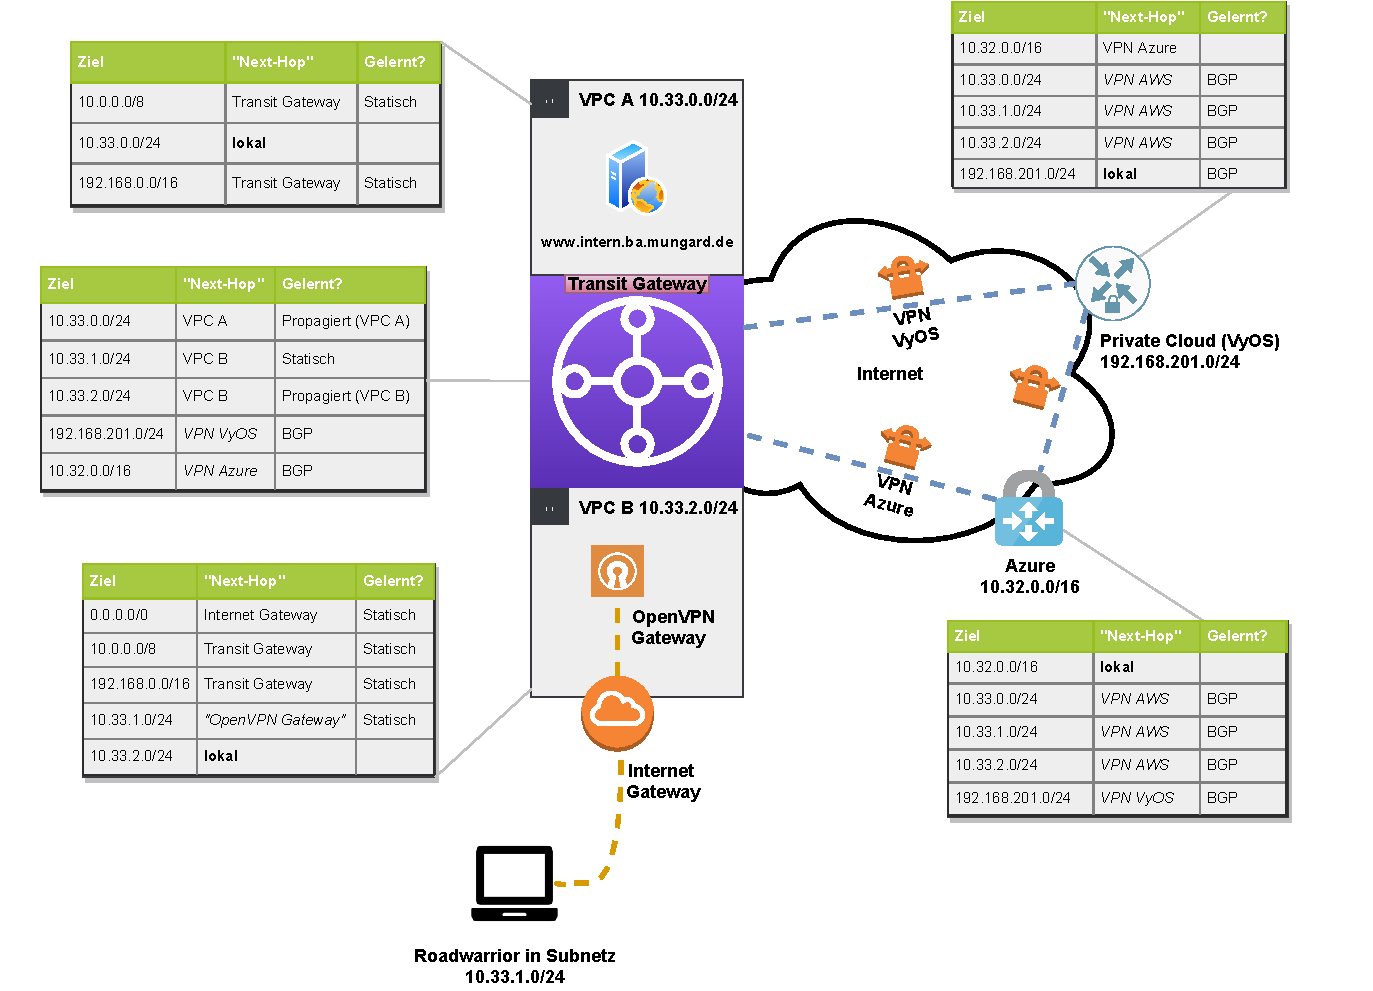
\includegraphics[scale=0.75]{Figures/Use-Case-2_AWS_TGW_Route-Tables.pdf}
  \caption{AWS Transit Gateway für Terminierung von VPN-Verbindungen und VPC-Peerings}
  \label{grafik:aws_tgw_route_tables}
\end{figure}\FloatBarrier
VPC CIDR und VPC Subnet werden in diesem Beispiel synonym verwendet, was formell nicht korrekt ist: Route Tables werden in Subnets genutzt, nicht im CIDR. Dies dient jedoch zur Vereinfachung des Schaubildes. Das Transit Gateway lernt die VPC CIDR automatisch, insofern \textit{Route Propagation} eingeschaltet ist.
\newpage
\subsection{Untersuchung von GeoIP-Daten}
Die GeoIP-Datenbank ist ein Binärformat\cite{maxmind2021binary}. Dies konnte durch das Werkzeug \texttt{file} nochmals bestätigt werden (\glqq data\grqq{})\cite{filemanpage2021}.
%TC:ignore
\begin{listing}[h]
\begin{minted}[breaklines,frame=single]{bash}
$ file /usr/share/GeoIP/GeoLite2-City.mmdb
/usr/share/GeoIP/GeoLite2-City.mmdb: data

\end{minted}
\caption{Auskunft über das Dateiformat mit \texttt{file}}
\label{file-geoip-db}
\end{listing}\FloatBarrier
%TC:endignore
Die Datensätze mussten \glqq sichtbar\grqq{} gemacht werden, um eine Idee zu bekommen, welche Spezifizierer genutzt werden können, um die DNS-Auflösung in regionaler Abhängigkeit umzusetzen. Weiterhin war nicht sichergestellt, welche Qualität die Datensätze aufweisen. Um dies zu testen, wurde ein kurzes Python-Skript \textit{mmdb.py} geschrieben und das Modul \textit{maxminddb} des GeoIP-Anbieters MaxMind eingebunden \cite{maxminddbreader2021}. Per \textit{pretty print} konnten die entsprechenden Datensätze für eine IP-Adresse ausgegeben werden.
%TC:ignore
\begin{listing}[h]
\begin{minted}[breaklines,frame=single]{python3}
#!/usr/bin/python3
import maxminddb
import sys
import pprint
print("++++++++++++++++++++ CITY INFO +++++++++++++++++++\n")
with maxminddb.open_database('/usr/share/GeoIP/GeoLite2-City.mmdb') as reader:
    pprint.pprint(reader.get(sys.argv[1]))
print("++++++++++++++++++++ CITY INFO +++++++++++++++++++\n")
#aehnliche Code-Teile ausgelassen
\end{minted}
\caption{Python-Skript mit Modul maxminddb zur Untersuchung der GeoIP-Datenbank}
\label{python-mmdb-reader}
\end{listing}\FloatBarrier
%TC:endignore
\newpage
Eine Beispielausgabe ist in Listing \ref{mmdb-example} für eine IP-Adresse der Fachhochschule Kiel zu sehen.
%TC:ignore
\begin{listing}[h]
\begin{minted}[breaklines,frame=single]{bash}
$ dig +short fh-kiel.de A
149.222.20.63

$ mmdb.py 149.222.20.63
++++++++++++++++++++ ASN INFO ++++++++++++++++++++

{'autonomous_system_number': 680,
 'autonomous_system_organization': 'Verein zur Foerderung eines Deutschen '
                                   'Forschungsnetzes e.V.'}
++++++++++++++++++++ ASN INFO ++++++++++++++++++++
[...]
++++++++++++++++++++ CITY INFO +++++++++++++++++++

{'city': {'geoname_id': 2891122,
          'names': {'de': 'Kiel',
                    'en': 'Kiel',
                    [...]
[...]
 'location': {'accuracy_radius': 20,
              'latitude': 54.3258,
              'longitude': 10.1379,
              'time_zone': 'Europe/Berlin'},
 'postal': {'code': '24149'},
[...]
++++++++++++++++++++ CITY INFO +++++++++++++++++++
\end{minted}
\caption{Beispielausgabe des Skripts mmdb.py}
\label{mmdb-example}
\end{listing}\FloatBarrier
%TC:endignore
Insgesamt erwiesen sich die Datensätze als sehr brauchbar und akkurat. Per cron-Job wird die Datenbank wöchentlich aktualisiert.

\subsection{Evaluation}

Es wurde pro Cloud-Standort eine virtuelle Maschine hochgefahren, die einen Roadwarrior-Client simulieren soll. Diese Clients haben \textbf{keinen} Zugriff auf interne Komponenten, sondern sind lediglich mit dem Internet verbunden, über welches VPN-Verbindungen zum jeweiligen VPN-Konzentrator aufgebaut werden können.

Nach dem \gls{Deployment} von Use-Case 2 wird geprüft, ob sich die Domain vpn.ba.mungard.de auflösen lässt. Dies wird demonstriert in Listing \ref{dns-resolution-client-vpn} für den Standort Azure Dublin.
%TC:ignore
\begin{listing}[h]
\begin{minted}[breaklines,frame=single]{bash}
ubuntu@vpn-client-azure:~$ dig +short vpn.ba.mungard.de A
94.245.93.144

\end{minted}
\caption{DNS-Auflösung für vpn.ba.mungard.de von Standort Azure (Dublin).}
\label{dns-resolution-client-vpn}
\end{listing}\FloatBarrier
%TC:endignore
Die IP-Adresse 94.245.93.144 gehört zu Microsoft.
%TC:ignore
\begin{listing}[h]
\begin{minted}[breaklines,frame=single]{bash}
$ whois 94.245.93.144 | grep mnt | uniq
mnt-by:         MICROSOFT-MAINT

\end{minted}
\caption{\texttt{whois} für die IP 94.245.93.144.}
\label{whois-microsoft-ip}
\end{listing}\FloatBarrier
%TC:endignore
Das Ziel ist ca. 1 Millisekunde entfernt. Für diesen Ping-Test wurde in der NSG manuell ICMP Echo Request erlaubt (eingehend). Im Standardfall würde für ICMP Echo Request ein \textit{Dropping} erfolgen.
%TC:ignore
\begin{listing}[h]
\begin{minted}[breaklines,frame=single]{bash}
ubuntu@vpn-client-azure:~$ ping 94.245.93.144
PING 94.245.93.144 (94.245.93.144) 56(84) bytes of data.
64 bytes from 94.245.93.144: icmp_seq=1 ttl=57 time=1.21 ms
64 bytes from 94.245.93.144: icmp_seq=2 ttl=57 time=0.936 ms
64 bytes from 94.245.93.144: icmp_seq=3 ttl=57 time=1.10 ms
64 bytes from 94.245.93.144: icmp_seq=4 ttl=57 time=1.04 ms
^C
--- 94.245.93.144 ping statistics ---
4 packets transmitted, 4 received, 0% packet loss, time 3003ms

rtt min/avg/max/mdev = 0.936/1.073/1.216/0.106 ms

\end{minted}
\caption{Ping von Roadwarrior-Client Azure $\rightarrow$ vpn.ba.mungard.de.}
\label{ping-microsoft-ip}
\end{listing}\FloatBarrier
%TC:endignore
Die Annahme von nun an ist, dass die lokale DNS-Auflösung auch für AWS funktioniert. Daher folgt an dieser Stelle nur ein Ping mit vorheriger Auflösung des Hostnamens vpn.ba.mungard.de. Die Round-Trip-Time (TTL) ist vergleichbar mit Azure (s. Listing \ref{ping-microsoft-ip}).
%TC:ignore
\begin{listing}[h]
\begin{minted}[breaklines,frame=single]{bash}
ubuntu@vpn-client-aws:~$ ping vpn.ba.mungard.de
PING vpn.ba.mungard.de (3.67.38.135) 56(84) bytes of data.
64 bytes from ec2-3-67-38-135.eu-central-1.compute.amazonaws.com (3.67.38.135): icmp_seq=1 ttl=63 time=0.930 ms
64 bytes from ec2-3-67-38-135.eu-central-1.compute.amazonaws.com (3.67.38.135): icmp_seq=2 ttl=63 time=1.16 ms
64 bytes from ec2-3-67-38-135.eu-central-1.compute.amazonaws.com (3.67.38.135): icmp_seq=3 ttl=63 time=0.970 ms
64 bytes from ec2-3-67-38-135.eu-central-1.compute.amazonaws.com (3.67.38.135): icmp_seq=4 ttl=63 time=0.947 ms
^C
--- vpn.ba.mungard.de ping statistics ---
4 packets transmitted, 4 received, 0% packet loss, time 3004ms
rtt min/avg/max/mdev = 0.930/1.001/1.157/0.091 ms

\end{minted}
\caption{Ping von Roadwarrior-Client AWS $\rightarrow$ vpn.ba.mungard.de.}
\label{ping-aws-ip}
\end{listing}\FloatBarrier
%TC:endignore
Es wurde eine virtuelle Maschine in der Public Cloud der Firma Hetzner am Standort Nürnberg bereitgestellt, welche einen Roadwarrior-Client simuliert, welcher an keinem der Standorte (Dublin, Frankfurtl, Kiel) verfügbar ist. Die Annahme ist, dass eine DNS-Anfrage die \glqq match-all\grqq-ACl treffen müsste, was Fall b) repräsentiert (vgl. Abb. \ref{grafik:Use-Case_2_Entscheidungsbaum_GeoIP}). Das \texttt{dig}-Kommando liefert drei A-Records für die Domain vpn.ba.mungard.de aus, somit wird diese ACL getroffen (s. Listing \ref{dig-match-all}).
%TC:ignore
\begin{listing}[h]
\begin{minted}[breaklines,frame=single]{bash}
root@openvpn-client:~# dig +short vpn.ba.mungard.de A
3.67.38.135
195.244.254.197
94.245.93.144

\end{minted}
\caption{\texttt{dig}-Kommando liefert drei A-Records}
\label{dig-match-all}
\end{listing}\FloatBarrier
%TC:endignore
\newpage
Weiterhin wurde getestet, ob Fall a) abgedeckt ist (vgl. Abb. \ref{grafik:Use-Case_2_Entscheidungsbaum_GeoIP}). Der VPN-Client in Azure Dublin verbindet sich mit dem lokal vorhandenen VPN-Konzentrator (s. Listing \ref{openvpn-connect-log}).
Der Filterausdruck mit \texttt{grep} ist für IPv4-Adressen und macht das Verbindungs-Log übersichtlicher. Analoge Tests waren für die anderen Cloud-Standorte erfolgreich.
%TC:ignore
\begin{listing}[h]
\begin{minted}[breaklines,frame=single]{text}
ubuntu@vpn-client-azure:~$ sudo openvpn --config config.ovpn 2>&1 | grep -E '(([0-9]{,3})\.){3}[0-9]{,3}'
Wed May 12 11:27:26 2021 TCP/UDP: Preserving recently used remote address: [AF_INET]94.245.93.144:61231
Wed May 12 11:27:26 2021 UDP link remote: [AF_INET]94.245.93.144:61231
Wed May 12 11:27:26 2021 TLS: Initial packet from [AF_INET]94.245.93.144:61231, sid=edbf2413 4ce1aa1c
Wed May 12 11:27:26 2021 [vpn-server-azure.ba.mungard.de] Peer Connection Initiated with [AF_INET]94.245.93.144:61231
Wed May 12 11:27:27 2021 PUSH: Received control message: 'PUSH_REPLY,dhcp-option DNS 192.168.201.1,route 10.32.0.0 255.255.0.0,route 10.33.0.0 255.255.0.0,route 192.168.201.0 255.255.255.0,dhcp-option DOMAIN intern.ba.mungard.de,route-gateway 10.32.1.1,topology subnet,ping 10,ping-restart 60,ifconfig 10.32.1.2 255.255.255.0'
Wed May 12 11:27:27 2021 ROUTE_GATEWAY 10.42.0.1/255.255.255.0 IFACE=eth0 HWADDR=00:0d:3a:dc:ec:4f
Wed May 12 11:27:27 2021 /sbin/ip addr add dev tun0 10.32.1.2/24 broadcast 10.32.1.255
Wed May 12 11:27:27 2021 /etc/openvpn/update-systemd-resolved tun0 1500 1557 10.32.1.2 255.255.255.0 init
May 12 11:27:27 update-systemd-resolved: Adding IPv4 DNS Server 192.168.201.1
Wed May 12 11:27:27 2021 /sbin/ip route add 10.32.0.0/16 via 10.32.1.1
Wed May 12 11:27:27 2021 /sbin/ip route add 10.33.0.0/16 via 10.32.1.1
Wed May 12 11:27:27 2021 /sbin/ip route add 192.168.201.0/24 via 10.32.1.1

\end{minted}
\caption{OpenVPN Verbindungs-Log des Roadwarrior-Clients}
\label{openvpn-connect-log}
\end{listing}\FloatBarrier
%TC:endignore
\newpage
Um den Fallback zu testen, wurde eine spezielle \texttt{iptables}-Regel eingerichtet, die ausgehende Pakete, in denen der String \glqq vpn\grqq{} enthalten ist, verwirft. \textit{vpn-default} bleibt hingegen erlaubt: Die Regel wird über der erstgenannten Regel ausgewertet (s. Listing \ref{iptables-deny-string-dns}).
%TC:ignore
\begin{listing}[h]
\begin{minted}[breaklines,frame=single]{bash}
$ sudo iptables-save | grep vpn
-A OUTPUT -p udp -m string --string "default-vpn" --algo bm --to 65535 -m udp --dport 53 -j ACCEPT
-A OUTPUT -p udp -m string --string "vpn" --algo bm --to 65535 -m udp --dport 53 -j DROP

\end{minted}
\caption{\texttt{iptables}-Filterregeln für DNS-Anfragen}
\label{iptables-deny-string-dns}
\end{listing}\FloatBarrier
%TC:endignore
Die Domain vpn.ba.mungard.de ist daraufhin nicht mehr auflösbar, default-vpn.ba.mungard.de hingegen schon (s. Listing \ref{dig-fail-vpn-fallback-to-default-vpn}).
%TC:ignore
\begin{listing}[h]
\begin{minted}[breaklines,frame=single]{bash}
ubuntu@vpn-client-azure:~$ dig +short vpn.ba.mungard.de A
;; connection timed out; no servers could be reached

ubuntu@vpn-client-azure:~$ dig +short default-vpn.ba.mungard.de A
195.244.254.197

\end{minted}
\caption{Funktionierende \texttt{iptables}-Filterregel für vpn.ba.mungard.de}
\label{dig-fail-vpn-fallback-to-default-vpn}
\end{listing}\FloatBarrier
%TC:endignore
Dies macht sich auch beim Verbindungsversuch mit OpenVPN bemerkbar. Ein Fallback auf die IP 195.244.254.197 erfolgt, da vpn.ba.mungard.de nicht mehr auflösbar ist (s. Listing \ref{connection-fail-vpn-fallback-default-vpn}). Die IP-Adresse entpricht dabei dem FQDN default-vpn.ba.mungard.de. Fall c) wurde somit erfolgreich abgebildet (vgl. Abb. \ref{grafik:Use-Case_2_Entscheidungsbaum_GeoIP}).
%TC:ignore
\begin{listing}[h]
\begin{minted}[breaklines,frame=single]{bash}
ubuntu@vpn-client-azure:~$ sudo openvpn --config config.ovpn 2>&1
Wed May 12 12:19:14 2021 RESOLVE: Cannot resolve host address: vpn.ba.mungard.de:61231 (Name or service not known)
Wed May 12 12:19:14 2021 RESOLVE: Cannot resolve host address: vpn.ba.mungard.de:61231 (Name or service not known)
Wed May 12 12:19:14 2021 Could not determine IPv4/IPv6 protocol
Wed May 12 12:19:14 2021 SIGUSR1[soft,init_instance] received, process restarting
Wed May 12 12:19:14 2021 Restart pause, 5 second(s)
Wed May 12 12:19:19 2021 UDP link remote: [AF_INET]195.244.254.197:61231
[...]
Wed May 12 12:19:20 2021 Initialization Sequence Completed

\end{minted}
\caption{OpenVPN-Verbindungsversucht mit \texttt{iptables}-Filterregel}
\label{connection-fail-vpn-fallback-default-vpn}
\end{listing}\FloatBarrier
%TC:endignore

Der Aufruf der Webseite \glqq http://www.intern.ba.mungard.de\grqq{} mit dem Textbrowser Lynx funktioniert. Somit wird immer der Server angesprochen, der am jeweiligen Cloud-Standort bereitgestellt wurde (s. Listing \ref{lynx-default-page}). Zeile 3 resultiert aus dem \texttt{sed}-Befehl (s. Listing \ref{sed-replace-apache-location}).
%TC:ignore
\begin{listing}[h]
\begin{minted}[linenos,breaklines,frame=single]{bash}
ubuntu@vpn-client-azure:~$ lynx -dump http://www.intern.ba.mungard.de | head -2
   Ubuntu Logo Apache2 Ubuntu Default Page
   It works! @Azure Cloud (Location: "North Europe - Dublin")

\end{minted}
\caption{Die Apache-Standardseite wird angezeigt..}
\label{lynx-default-page}
\end{listing}\FloatBarrier
%TC:endignore
Alle hier geschilderten Tests waren analog für alle weiteren Roadwarrier-Clients und Cloud-Standorte erfolgreich und es konnten somit alle Evaluationskriterien von Use-Case 2 erfüllt werden (siehe \ref{eval-roadwarrior}).\\
Auch zusammenfassend ist zu sagen, dass eine erfolgreiche Demonstration beider Use-Cases stattgefunden hat und die technischen Kapitel damit abgeschlossen sind. Im folgenden Kapitel \ref{Fazit und Ausblick} erfolgt eine abschließende Betrachtung der Arbeit mit Fazit und Ausblick.